\subsection{Switch sizing} \label{switch_sizing}

The system must regulate the energy flow in order to maximize the energy generation. In order to achieve this, the system includes switches that control the current flow. The switches consist on MOSFET devices. The switching frequency of the system is $50 $ kHz. Although the market has IGBT which can switch at $50$ kHz, MOSFET devices allow lower losses than IGBTs for system's current rating. \cite{mosfet_igbt_switching_loss} \cite{igbt_or_mosfet}

The maximum output voltage of the system is $90 $V, however the voltage rating of the transistors was set to $150 $V in order to increase the reliability. The peak current through the transistors happens when the buck mode is activated. The peak current is equal to $14$ A. In order to reduce the conduction losses and the heat sink size, a low on resistance is desired. This constraints were used when searching for the ideal component. The chosen device is the IPB200N15N3GATMA1. It exhibits the features seen in table \ref{mosfet_features}.

\begin{table}[htbp]
	\centering
	\begin{tabular}{|p{6cm}|>{\centering}p{8cm}|}
		\hline
		\rowcolor{lightgray}\multicolumn{2}{|l|}{ \textbf{Maximum ratings}} \\ \hline
		Continuous $I_{D}$ & 40 [A]  \tabularnewline \hline
		$V_{GS}$ & $\pm$ 20 [V]  \tabularnewline \hline
		Power dissipation & 150 [W]  \tabularnewline \hline
		$V_{DS}$ & 150 [V]  \tabularnewline \hline
		$R_{DSon} $ & 20 [m$\Omega$]  \tabularnewline \hline
		\rowcolor{lightgray}\multicolumn{2}{|l|}{ \textbf{Other values of interest}} \\ \hline
		$C_{GS} $ & 1.81 [nF]  \tabularnewline \hline
		Package & D2PAK  \tabularnewline \hline
	
	\end{tabular}
	\caption{MOSFET figures of merit. T = 25 $\decC$. \cite{mosfet_datasheet}}
	\label{mosfet_features}
\end{table}

The power dissipated in the switches is equal to the sum of the conduction losses and the switching losses. The conduction loss might be calculated  as seen in \ref{conduction_losses_eq}.

\begin{equation} \label{conduction_losses_eq}
P_{cond} = i(t)^2 \cdot R_{DS}
\end{equation}


The switching losses depend upon the switching frequency and the transistor's manufacturing characteristics. In order to calculate the value, the MOSFET's SPICE model was obtained from the manufacturer's website. The next step was to perform the simulation of the system. The system was simulated in both Buck and Boost modes. Special attention was put into the dead-band between PWM signals of different switches, to avoid current shoot through. After simulating, the average power dissipation under steady state was calculated in both Buck and Boost modes. Within every mode, the simulation was performed under the most unfavorable conditions, this is: Buck's output is 24 V and Boost's output is 90 V. The results can be seen in table \ref{mosfet_power_consumption}.


$R_{DS}$ is mainly dependant on the temperature. The models found neglect the temperature difference. Then, in order to get an approximated value considering temperature, the procedure will be to calculate the total losses at constant temperature using the SPICE model and then add the additional conduction losses due to the increase of the resistance, as expressed by equation \ref{total_losses}.

\begin{equation} \label{total_losses}
\overline{P} = \overline{P_{loss, T = K}} + \overline{i(t)^2} \cdot \Updelta R_{DS}
\end{equation}

Now the junction temperature based on the power dissipation calculated using the SPICE model is calculated:

\begin{equation} \label{switch_temperature}
T_{J} = T_{housing} + \overline{P_{loss, T = K}} + \cdot  R_{thermal}
\end{equation}

\begin{equation} \label{switch_temperature_w_values}
T_{J} = 40 + 5.54 \cdot  2.06 = 51.41 \decC
\end{equation}
Now the average current values was obtained from the system's simulation
\todo{Ahora se calcula la corriente media y se multiplica por rds a los 51 grados recien calculados, la cosa es que se tiene que comprobar que la corriente que se coja sea la de buck, ya que se cogio la potencia media del buc ya que era la mas elevada. Ahora el proceso a hacer es coger las dos corrientes medias, multiplicar por rds y sumar a la temperatura (al loro que habra 2 temperaturas no una) y coger el maximo para cerciorarse de que se estan cogiendo los valores adecuados. }
\begin{figure}[htbp]
	\begin{center}
		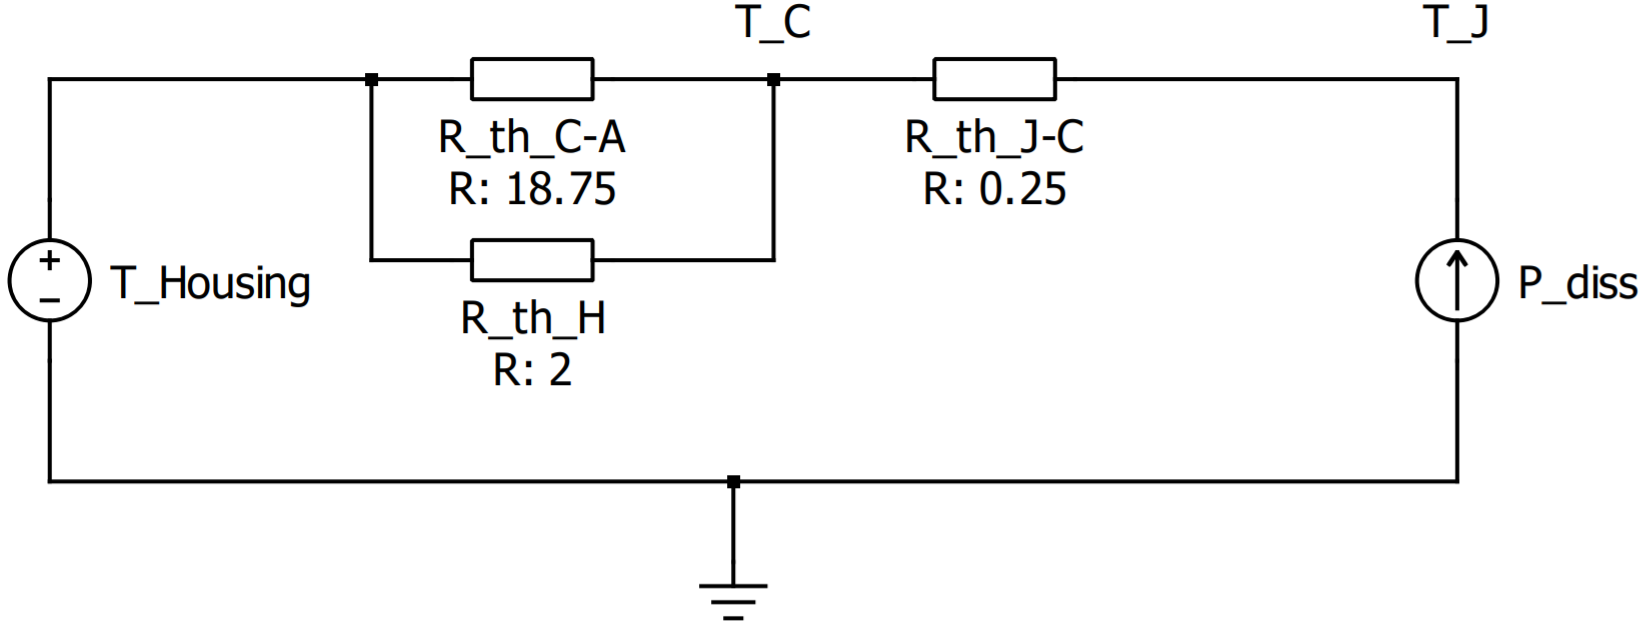
\includegraphics[width=0.4\textwidth]{../Pictures/thermal_circuit.png}
		\caption{Thermal circuit used for sizing the heat sink}
		\label{thermal_circuit}
	\end{center}	
\end{figure}



\begin{table}[htbp]
	\centering
	\begin{tabular}{|p{6cm}|>{\centering}p{8cm}|}
		\hline
		\rowcolor{lightgray}\multicolumn{2}{|l|}{ \textbf{Buck Mode}} \\ \hline
		M1 & 2.91 [W]  \tabularnewline \hline
		M2 & 0.82 [W]  \tabularnewline \hline
		M3 & 1.81 [W]  \tabularnewline \hline
		M4 & 0 [W]  \tabularnewline \hline
		Total & 5.54 [W]  \tabularnewline \hline
		\rowcolor{lightgray}\multicolumn{2}{|l|}{ \textbf{Boost Mode}} \\ \hline
		M1 & 0.69 [W]  \tabularnewline \hline
		M2 & 0 [W]  \tabularnewline \hline		
		M3 & 0.48 [W]  \tabularnewline \hline
		M4 & 3.31 [W]  \tabularnewline \hline
		Total & 4.48 [W]  \tabularnewline \hline
		
	\end{tabular}
	\caption{Average power dissipation in every MOSFET.}
	\label{mosfet_power_consumption}
\end{table}

When the power dissipation values are known

